\documentclass{standalone}
\usepackage{tikz}

\begin{document}
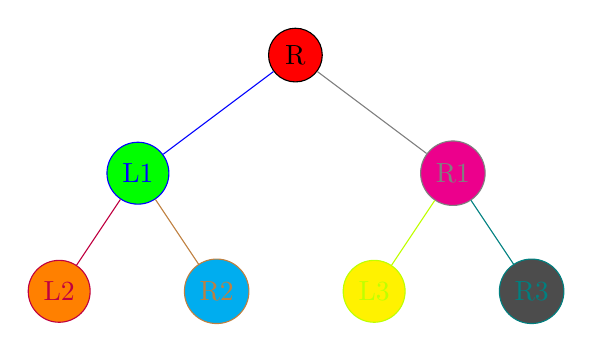
\begin{tikzpicture}[level distance=1.5cm,
                    level 1/.style={sibling distance=4cm},
                    level 2/.style={sibling distance=2cm},
                    level 3/.style={sibling distance=1cm}]
    \node (root) [circle, draw, fill=red] {R}
        child [color=blue] {
            node (left1) [circle, draw, fill=green] {L1}
                child [color=purple] {
                    node (left2) [circle, draw, fill=orange] {L2}
                }
                child [color=brown] {
                    node (right2) [circle, draw, fill=cyan] {R2}
                }
        }
        child [color=gray] {
            node (right1) [circle, draw, fill=magenta] {R1}
                child [color=lime] {
                    node (left3) [circle, draw, fill=yellow] {L3}
                }
                child [color=teal] {
                    node (right3) [circle, draw, fill=black!70] {R3}
                }
        };
\end{tikzpicture}
\end{document}